% this file is called up by thesis.tex
% content in this file will be fed into the main document

\chapter{The Data} % top level followed by section, subsection
\label{cha:data}

% ----------------------- contents from here ------------------------

At the time of undertaking this project, the KM3NeT Neutrino Telescope
was still under construction, thus simulated data provided by Nikhef
was used. The data itself was provided in two parts namely
\emph{events} and \emph{noise} datasets, both of which came from
different sources and in different formats. The events dataset was
provided as a 42MB \emph{HDF5} (Hierarchical Data Format) file
consisting of the \emph{/data/mc\_hits} and \emph{/data/mc\_info}
tables. For the purposes of this project, the two tables were combined
such that each row in the mc\_hits table contains its corresponding
'event\_id' from the mc\_info table. A \emph{label} column was added
containing a value of '1' and the resulting table (henceforth referred
to as the \emph{events} dataset) was saved as a CSV file.

The \emph{noise} data was generated using a Python library implemented
and maintained by Nikhef, \emph{k40gen}.
\texttt{k40gen.Generators(21341, 1245, [7000., 700., 70., 0.])} was
used to create an instance of a generator where the first two
arguments are random seeds followed by a list of rates at which
single, double, triple and quadruple hits should be generated. The
generator instance is then passed into \texttt{k40gen.generate\_40()}
method which returns a (4, n) array containing as rows \emph{time
(t)}, \emph{dom\_id}, \emph{pmt\_id} and \emph{time over threshold
(tot)}). The position coordinates (ie. \emph{x}, \emph{y} and \emph{z}
coordinates) for each datapoint was provided in a
\emph{positions.detx} file which was parsed using the Numpy Python
package \cite{numpy} and added to the \emph{noise} array. The Python
library Pandas \cite{pandas} was used to convert the array into a (n,
4) dataframe. A \texttt{label} column was added containing a value of
'0' and the dataframe was saved as a 3.9GB CSV file.

To create the \emph{main} dataset for the project, the events and
noise datasets were combined. Both datasets were read into memory as
Pandas dataframes and their columns were renamed for consistency. The
two dataframes were concatenated and sorted based on the time column.
Rows with negative time were dropped along with columns which were not
relevant to this project. The \texttt{time} column was discretised
into 15000ns bins and the resulting values were added to the
\texttt{timeslice} column. The resulting dataframe was saved as a
1.9GB CSV file. The main dataset was explored using statistical
analysis and visualizations to observe any patterns and ``local
trends'' that may be present. Due to the high number of data points, a
random sample of 10\% of the data was taken in order to draw
reasonable conclusions from the plots.

\begin{table}[h]
  \centering
  \caption{Description of columns}
  \label{tab:desc-cols}
  \begin{tabular}{p{1.5cm}p{1.5cm}p{2cm}p{8cm}}
    \hline
    Column & Data type & Unit & Description \\
    \hline
    x, y, z & float & meters (m) & The position within the detector
    where the hit was detected, they represent the x,y,z coordinates
    of the hit respectively. \\
    t & float & nano seconds (ns) & The time at which the hit was
    detected. \\
    label & int & NA & The type of hit, '0' represents noise and '1'
    represents a neutrino hit \\
    event\_id & int & NA & The id of the event to which the hit is
    related to. The id itself does not have any meaning, it is simply
    used to identify hits that originated from the same event. \\
    timeslice & int & NA & The id of the timeslice to which the hit
    belongs. The id itself does not have any meaning, it is simply
    used to group hits into discrete bins. \\
    \hline
  \end{tabular}
\end{table}

Table \ref{tab:desc-stats} presents the descriptive statistics of the
dataset. The dataset consists of 7 columns (or features) and roughly
4.5 million rows. Table \ref{tab:desc-cols} provides more information
on the columns of the dataset. The dataset does not contain any
\texttt{nan} or \texttt{null} values except for the \texttt{event\_id}
column where rows containing noise hits are not associated with any
event. Next, the correlations amongst the features are checked using
the "Pearson" correlation and depicted by a correlation matrix in
Figure \ref{fig:corr}. No significant correlations are observed
between \emph{x}, \emph{y}, \emph{z} and \emph{t} which indicates that
ML models may not be able to learn anything from the dataset without
the aid of feature engineering. The distribution of the \texttt{label}
column is presented in Figure \ref{fig:dist-label}. A severe class
imbalance was noted between events and noise hits. The dataset
contains 489906 instances of events compared to over 4 million
instances of noise. An effective strategy to handle the class
imbalance was devised during training of models to prevent
\emph{overfitting}.

\begin{figure}[htb]
  \begin{minipage}[t]{0.64\textwidth}
  \centering
  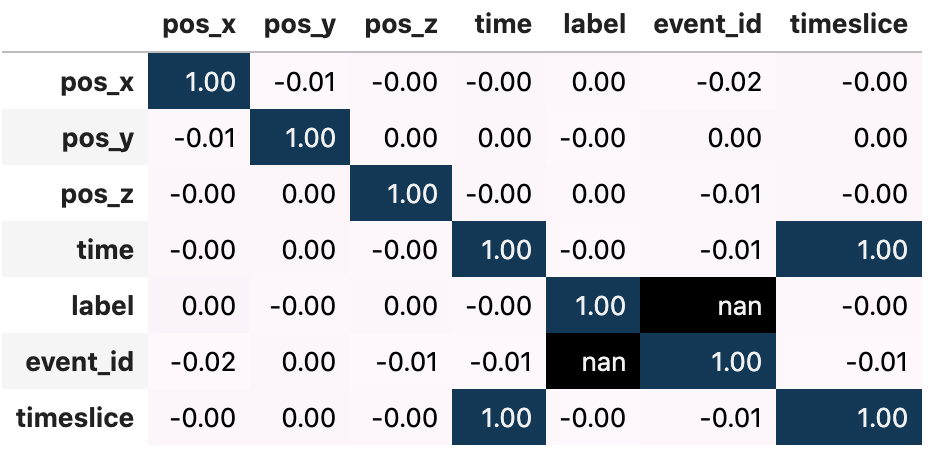
\includegraphics[width=\linewidth]{correlation.png}
  \caption{Correlation matrix of features}
  \label{fig:corr}    
  \end{minipage}
  \begin{minipage}[t]{0.34\textwidth}
  \centering
  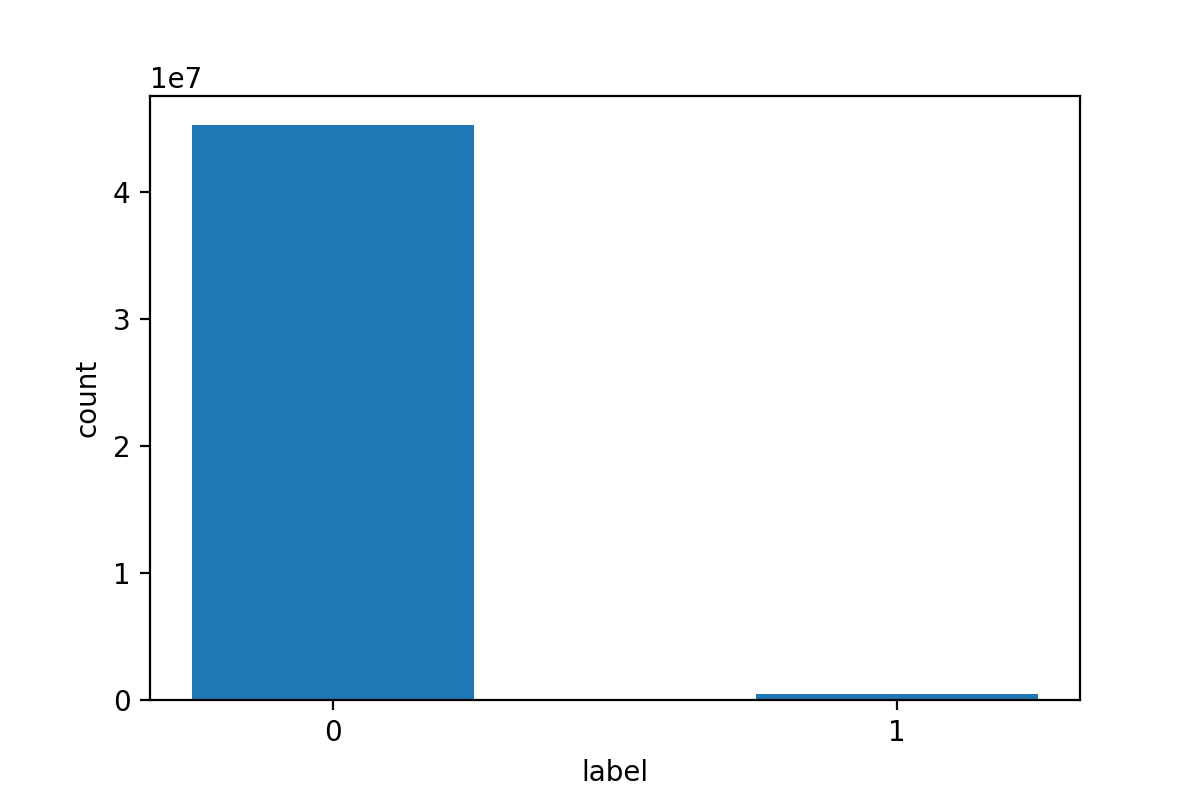
\includegraphics[width=\linewidth]{dist-label.png}
  \caption{Distribution of \texttt{label} column}%
  \label{fig:dist-label}    
  \end{minipage}
\end{figure}

\begin{table}[htb]
  \centering
  \caption{Descriptive statistics}
  \label{tab:desc-stats}
  \begin{tabular}{lrrrrrrr}
    \hline
          & x & y & z & t & label & event\_id & timeslice \\
    \hline
    count & 4.58e+7 &  4.58e+7 &  4.58e+7 &  4.58e+7 &  4.58e+7 &  489906 &  4.58e+7 \\
    mean  & 1.16e-02 & -1.59e-02 &  1.17e+02 &  5.00e+07 &  1.06e-02 &    2862.00 &  3.33e+03 \\
    std   & 5.12e+01 &  6.22e+01 &  4.86e+01 &  2.89e+07 &  1.02e-01 &    1667.61 &  1.92e+03 \\
    min   & -9.46e+01 & -1.15e+02 &  3.77e+01 &  0.00e+00 &  0.00e+00 &       0.00 &  0.00e+00 \\
    25\%  & -4.50e+01 & -5.79e+01 &  7.40e+01 &  2.50e+07 &  0.00e+00 &    1392.25 &  1.66e+03 \\
    50\%  & 1.30e+00 & -4.18e+00 &  1.21e+02 &  5.00e+07 &  0.00e+00 &    2887.00 &  3.33000e+03 \\
    75\%  & 4.04e+01 &  4.85e+01 &  1.60e+02 &  7.50e+07 &  0.00e+00 &    4304.75 &  5.00000e+03 \\
    max  & 9.62e+01 &  1.05e+02 &  1.96e+02 &  1.01e+08 &  1.00e+00 &    5734.00 &  6.77e+03 \\
    \hline
  \end{tabular}
\end{table}

The dataset is derived from synthetically generated data using
simulations. As such, it is likely that the event hits in each
timeslice may occur at a specific time such as at the beginning,
middle or end of the timeslice. Having such a pattern in the dataset
may bias the model since it may learn this pattern and thus fail to
generalize. If this pattern does exist in the dataset, corrective
measures need to be taken such that the event hits in each timeslice
are uniformly distributed. To verify the existence of such patterns in
the dataset, the mean time of event hits across all events was
visualized as a scatter plot as depicted by Figure
\ref{fig:bias-verification}. A uniform distribution is noted with no
visible patterns indicating no bias exists in the dataset and it is
deemed suitable for further analysis.

 \begin{figure}[htb]
   \begin{minipage}{0.32\textwidth}
     \centering
     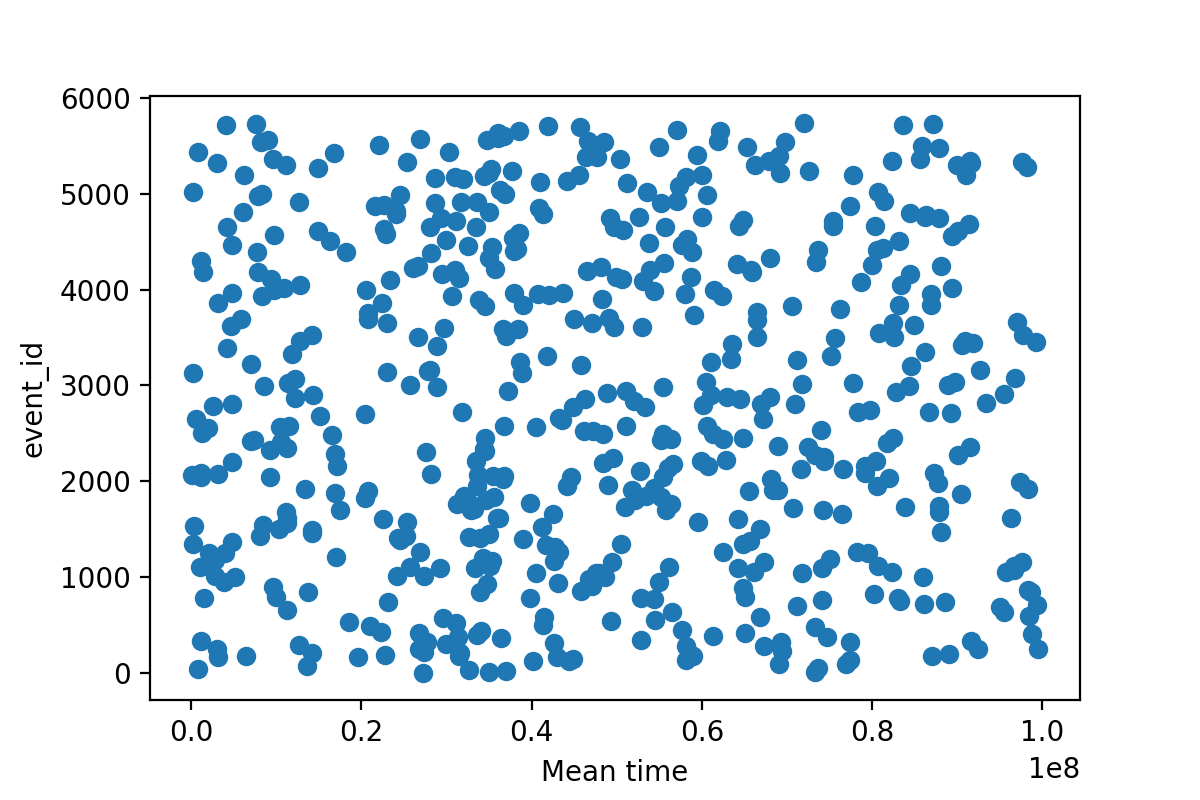
\includegraphics[width=\linewidth]{bias-verification.png}
     \caption{Verification of Bias}%
     \label{fig:bias-verification}     
   \end{minipage}
   \begin{minipage}{0.32\textwidth}
     \centering
     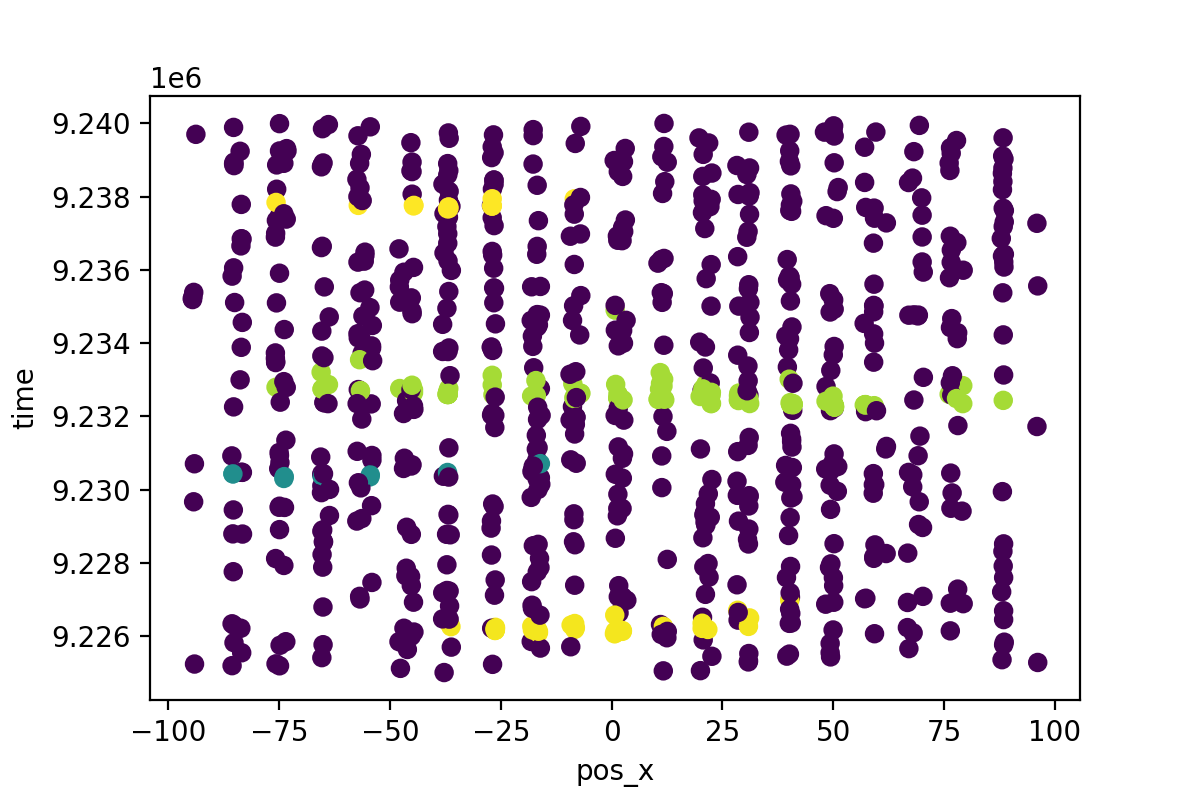
\includegraphics[width=\linewidth]{dist-timeslice-largest-posx-time-eventid.png}
     \caption{Distribution of Timeslice 615}%
     \label{fig:dist-timeslice-largest}    
   \end{minipage}
   \begin{minipage}{0.32\textwidth}
     \centering
     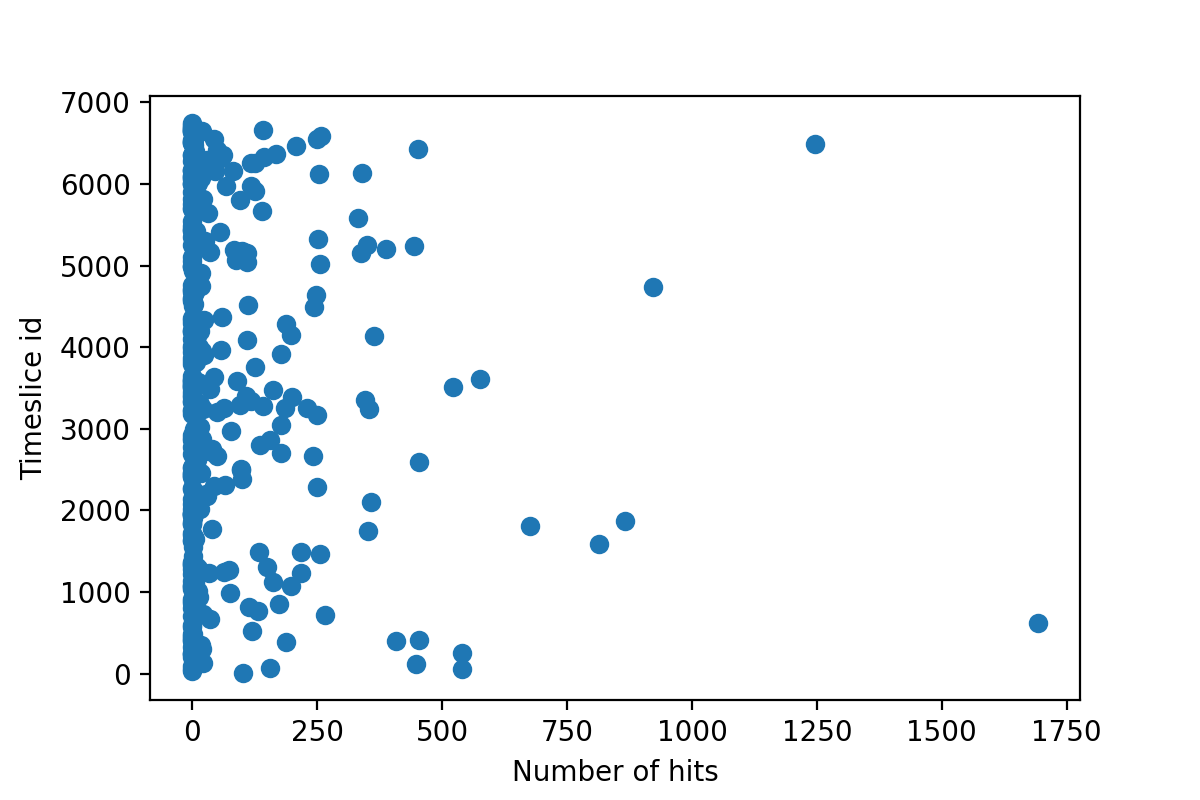
\includegraphics[width=\linewidth]{dist-hits-per-timeslice.png}
     \caption{Distribution of event hits per timeslice}%
     \label{fig:dist-hits-per-timeslice}    
   \end{minipage}
 \end{figure}

 The dataset is discretized into 6759 timeslices of which 2783
 timeslices contain only noise hits. This is corroborated by Figure
 \ref{fig:dist-hits-per-timeslice} which presents a skewed
 distribution where many timeslices contain few to no event hits and
 few timeslices contain a high number of event hits. Figure
 \ref{fig:dist-timeslice-largest} depicts a scatter plot of
 \emph{timeslice 615} which contains the largest number of event hits.
 It is observed that event hits occur close to each other in space and
 time (represented by the yellow, blue and green points) whilst
 background hits are uniformly distributed in space and time
 (represented by the purple points).

 % ---------------------------------------------------------------------------
 % ----------------------- end of thesis sub-document ------------------------
 % ---------------------------------------------------------------------------
